
% Inbuilt themes in beamer
\documentclass[aspectratio=169]{beamer}
\usepackage{graphicx}
% Theme choice:
\usetheme{CambridgeUS}

% Title page details: 
\title{Chapter 14: Firms in Competitive Markets} 
\author{Discussion section 4}
\date{April 2023}

\begin{document}

% Title page
\begin{frame}
    \titlepage 
\end{frame}

% Outline frame
\begin{frame}{Outline}
    \begin{itemize}
        \item We now have our tools: marginal product, marginal cost, average total cost, total profit \dots
        \item We will now consider firms in a \textit{competitive marketplace} which have no \textit{market power}
        \item We will figure out how firms choose output, and see a surprising equilibrium result
    \end{itemize}
\end{frame}

\begin{frame}{Competitive market}
    \begin{itemize}
        \item Competitive market means:
    \end{itemize}
\end{frame}

\begin{frame}{Competitive market}
    \begin{itemize}
        \item Competitive market means:
            \begin{itemize}
                \item There are a ``large'' number of buyers
                \item Product is undifferentiated
                \item All actors are price-takers
            \end{itemize}
        \item We will add \textit{free entry and exit}: firms can move in and out of production at 0 cost
        \item What do these conditions mean for a firm's total revenue? What about for its marginal revenue?
    \end{itemize}
\end{frame}

\begin{frame}{Average}
    \begin{itemize}
        \item What do these conditions mean for a firm's total revenue? 
            \begin{itemize}
                \item Remember: TR = P * Q
            \end{itemize}
        \item AR = $\frac{TR}{Q}$ = P
        \item What about for its marginal revenue? 
    \end{itemize}
\end{frame}

\begin{frame}{Marginal revenue}
    \begin{itemize}
        \item What do these conditions mean for a firm's total revenue? 
            \begin{itemize}
                \item Remember: TR = P * Q
            \end{itemize}
        \item AR = $\frac{TR}{Q}$ = P
        \item What about for its marginal revenue?
        \begin{itemize}
            \item Since the firm does not change the market price with its production decision, P is constant, thus the marginal revenue is also constant and MR = P
        \end{itemize}
    \end{itemize}
\end{frame}

\begin{frame}{Profit maximization}
    \begin{itemize}
        \item We know firms will choose output to maximize their profit
        \item How do they choose this point?
    \end{itemize}
\end{frame}

\begin{frame}{Profit maximization}
    \begin{itemize}
        \item We know firms will choose output to maximize their profit
        \item How do they choose this point?
            \begin{itemize}
                \item By \textit{thinking at the margin}
                \item They will keep producing more output until an additional unit causes their profit to decrease: ie until \textit{marginal profit} is 0
            \end{itemize}
    \end{itemize}
\end{frame}

\begin{frame}{Marginal profit}
    \begin{itemize}
        \item Marginal profit = change in profit from a ``small'' change in output
            \begin{itemize}
                \item Remember: profit = revenue - cost
                \item So marginal profit = marginal revenue - marginal cost
            \end{itemize}
        \item Marginal revenue is constant, but we saw that marginal cost is not, so marginal profit will not be either
        \item Producing up to 0 marginal profit means that MR = MC, which means P = MC
    \end{itemize}
\end{frame}

\begin{frame}{Optimal output}
    \centering
    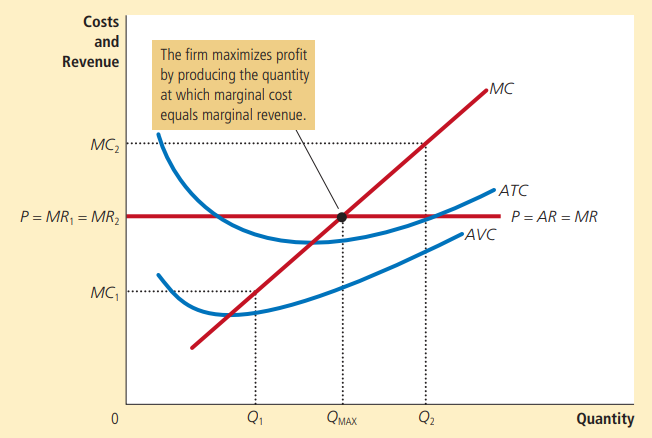
\includegraphics[width = 0.5\textwidth,keepaspectratio]{MReMC.png}
\end{frame}

\begin{frame}{Supply curve}
    \begin{itemize}
        \item Since marginal cost determines output, the MC cruve is the competitive firm's supply curve
    \end{itemize}
\end{frame}

\begin{frame}{Market entry}
    \begin{itemize}
        \item Firms can move out of the market in two ways: \textit{shutdown} or \textit{exit}
            \begin{itemize}
                \item A \textit{shutdown} is short-term: still have to pay fixed costs (eg rent)
                \item An \textit{exit} is long-term: don't pay fixed costs
            \end{itemize}
        \item In the short run, fixed costs are \textit{sunk costs}
        \item So, what do firms consider when deciding to shutdown?
    \end{itemize}
\end{frame}

\begin{frame}{Shutdown}
    \begin{itemize}
        \item So, what do firms consider when deciding to shutdown?
            \begin{itemize}
                \item They consider their \textit{variable costs}
                \item So the competitive firm’s short-run supply curve is the portion of its marginal-cost curve that lies above average variable cost
            \end{itemize}
        \item What do firms consider when deciding to exit?
    \end{itemize}
\end{frame}

\begin{frame}{Exit}
    \begin{itemize}
        \item What do firms consider when deciding to exit?
            \begin{itemize}
                \item \textit{Total} costs: shutdown if TR < TC
            \end{itemize}
        \item So, the long-run supply curve is the portion of the MC curve above ATC
    \end{itemize}
\end{frame}

\begin{frame}{Supply curves}
    \centering
    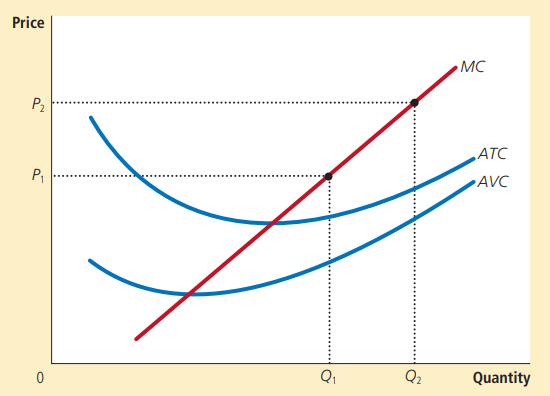
\includegraphics[width = 0.5\textwidth,keepaspectratio]{supply.png}
\end{frame}

\begin{frame}{Profit}
    \centering
    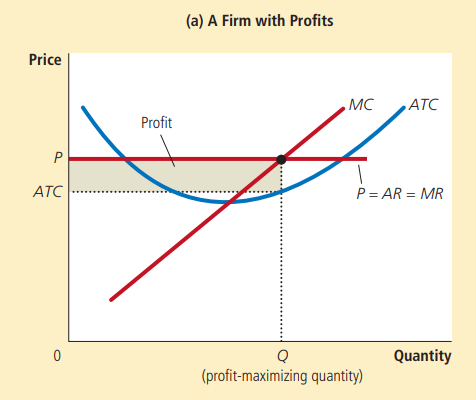
\includegraphics[width = 0.5\textwidth,keepaspectratio]{profit.png}
\end{frame}

\begin{frame}{Entry}
    \begin{itemize}
        \item The flip side is that firms will \textit{enter} if their ATC < MC
        \item Although the decision of an individual firm does not affect the price, ``many'' firms entering will expand Q and decrease P
            \begin{itemize}
                \item Many firms exiting, on the other hand, will decrease Q and increase P
            \end{itemize}
        \item At the end of this proccess, firms must be making \textit{zero economic profits}
            \begin{itemize}
                \item At this point, P = ATC
                \item All firms are operating at their ``efficient scale'', the minimum of ATC
            \end{itemize}
    \end{itemize}
\end{frame}

\begin{frame}{A shift in demand}
    \begin{itemize}
        \item Suppose that there is a shift in demand so that demand increases:
            \begin{itemize}
                \item What happens to the market price?
                \item What happens to profits?
                \item How will firms respond?
            \end{itemize}
    \end{itemize}
\end{frame}

\begin{frame}{A shift in demand}
    \begin{itemize}
        \item Suppose that there is a shift in demand so that demand increases:
            \begin{itemize}
                \item What happens to the market price? \textbf{The price increase.}
                \item What happens to profits? \textbf{Profits become positive.}
                \item How will firms respond? \textbf{New firms enter the market.}
            \end{itemize}
        \item How does this effect the market?
    \end{itemize}
\end{frame}

\begin{frame}{A shift in demand}
    \begin{itemize}
        \item Increase in demand $\to$ higher P $\to$ positive profit $\to$ firm entry
        \item How does this effect the market?
            \begin{itemize}
                \item Firms enter the market
                \item This increases supply and decreases P
                \item P decreases until P = ATC Again
                \item Equilibrium is restored
            \end{itemize}
    \end{itemize}
\end{frame}

\begin{frame}{Long-run firm behavior}
    \begin{itemize}
        \item In the long run, the market supply curve is horizontal (perfectly elastic)
        \item In reality, why might curves may slope upwards?
    \end{itemize}
\end{frame}

\begin{frame}{Long-run firm behavior}
    \begin{itemize}
        \item In the long run, the market supply curve is horizontal (perfectly elastic)
        \item In reality, why might curves may slope upwards?
            \begin{itemize}
                \item Inputs may be limited
                \item Firms may have different costs
            \end{itemize}
    \end{itemize}
\end{frame}

% From this analysis of firm behavior, we can determine the long-run supply curve for the market. In a market with free entry and exit, there is only one price consistent with zero profit—the minimum of average total cost. As a result, the long-run market supply curve must be horizontal at this price, as illustrated by the perfectly elastic supply curve in panel (b) of Figure 7
% demand curve shifts; new short-run equilibrium; eventual long-run equilibrium
% . Because firms can enter and exit more easily in the long run than in the short run, the long-run supply curve is typically more elastic than the short-run supply curve.




\end{document}
